\documentclass[11pt,a4paper]{article}
\usepackage[T1]{fontenc}
\usepackage[utf8]{inputenc}
\usepackage[magyar]{babel}
\usepackage{lmodern}
\usepackage{amsmath}
\usepackage{enumitem}
\usepackage{tikz}
\usepackage[a4paper,margin=2cm]{geometry}

\pagestyle{empty}
\setlength{\parindent}{0pt}

\begin{document}

\begin{center}
{\large\bfseries Termodinamika -- állapotjelzők és folyamatjellemzők\\[2pt]
megoldókulcs}

\vspace{6pt}
\fbox{\parbox{0.92\linewidth}{\centering
$\Delta E = Q + W$, ahol $W$ a \emph{gázon végzett} munka.}}
\end{center}

\vspace{2pt}

\begin{enumerate}[leftmargin=*,label=\textbf{\arabic*.},itemsep=9pt,topsep=0pt,parsep=0pt]

\item \textbf{a)} Igen, munkavégzéssel. Ha a gázt (pl.\ hőszigetelt hengerben) gyorsan
összenyomjuk, akkor $Q = 0$, $W > 0$, így $\Delta E = W > 0$, a hőmérséklet nő
(biciklipumpa). Súrlódással, keveréssel végzett munka is melegít.

\textbf{b)} Igen. Két példa:
\begin{itemize}[nosep,leftmargin=1.5em]
  \item \emph{Izoterm tágulás:} a gáz a felvett hővel egyenlő munkát végez a
    környezetén ($Q = -W > 0$, $\Delta E = 0$), így $T$ nem változik.
  \item \emph{Halmazállapot-változás:} olvadó jég ($0\,^\circ$C) vagy forrásban lévő víz
    ($100\,^\circ$C): a közölt hő a halmazállapot megváltoztatására fordítódik,
    a hőmérséklet állandó marad.
\end{itemize}

\item \textbf{Kulcsmegfigyelés:} $p_AV_A = p_0V_0$ és $p_BV_B = \tfrac{p_0}{2}\cdot 2V_0 =
p_0V_0$, tehát $T_A = T_B$.

\textbf{a)} A munka csak az izobár szakaszon nem nulla ($W = -p\,\Delta V$).
\begin{itemize}[nosep,leftmargin=1.5em]
  \item \textbf{I.~út:} $W_\text{I} = -p_0\cdot V_0 = -p_0V_0$ (az izochor szakaszon
    $W = 0$). $\;Q_\text{I} = \Delta E - W_\text{I} = 0 + p_0V_0 = p_0V_0$.
  \item \textbf{II.~út:} $W_\text{II} = -\tfrac{p_0}{2}\cdot V_0 = -\tfrac12 p_0V_0$.
    $\;Q_\text{II} = \Delta E - W_\text{II} = \tfrac12 p_0V_0$.
\end{itemize}

\textbf{b)} $\Delta E = 0$ mindkét úton, mert ideális gáz belső energiája csak a
hőmérséklettől függ, és $T_A = T_B$.

\textbf{c)} $W$ és $Q$ függ az úttól (folyamatjellemzők), $\Delta E$ nem
(a belső energia állapotjelző: csak a kezdő- és végállapot határozza meg). Az ábrán a
munka a görbe alatti terület, ez a két úton eltérő.

\emph{Kiegészítés (szakaszonként, egyatomos gázra, $E = \tfrac32 pV$), $p_0V_0$
egységben:}
\begin{center}
\renewcommand{\arraystretch}{1.3}
\begin{tabular}{|l|c|c|c|}
\hline
Szakasz & $W$ & $\Delta E$ & $Q$ \\ \hline
I.\ izobár tágulás ($p_0$)          & $-1$ & $+\tfrac32$ & $+\tfrac52$ \\
I.\ izochor hűtés ($2V_0$)           & $0$ & $-\tfrac32$ & $-\tfrac32$ \\ \hline
II.\ izochor hűtés ($V_0$)           & $0$ & $-\tfrac34$ & $-\tfrac34$ \\
II.\ izobár tágulás ($p_0/2$)       & $-\tfrac12$ & $+\tfrac34$ & $+\tfrac54$ \\ \hline
\end{tabular}
\end{center}

\item A kitöltött táblázat:
\begin{center}
\renewcommand{\arraystretch}{1.5}
\begin{tabular}{|l|c|c|c|c|}
\hline
\textbf{Folyamat} & \hspace{0.5cm}$\Delta T$\hspace{0.5cm} & \hspace{0.5cm}$\Delta E$\hspace{0.5cm}
  & \hspace{0.5cm}$W$\hspace{0.5cm} & \hspace{0.5cm}$Q$\hspace{0.5cm} \\ \hline
izoterm tágulás         & $0$ & $0$ & $-$ & $+$ \\ \hline
izochor melegítés       & $+$ & $+$ & $0$ & $+$ \\ \hline
adiabatikus összenyomás & $+$ & $+$ & $+$ & $0$ \\ \hline
\end{tabular}
\end{center}
\textbf{Indoklások:}
\begin{itemize}[nosep,leftmargin=1.5em]
  \item \emph{Izoterm tágulás:} $\Delta T = 0$ a folyamat definíciója szerint;
    $\Delta E = 0$, mert $E$ csak $T$-től függ; $W < 0$, mert a gáz tágul, ő végez
    munkát; $Q = -W > 0$ az I.~főtétel szerint.
  \item \emph{Izochor melegítés:} $\Delta T > 0$, mert melegítjük; $\Delta E > 0$, mert
    $T$ nő; $W = 0$, mert a térfogat nem változik; $Q = \Delta E > 0$.
  \item \emph{Adiabatikus összenyomás:} $Q = 0$ definíció szerint; $W > 0$, mert mi
    nyomjuk össze a gázt; $\Delta E = W > 0$; ezért $\Delta T > 0$.
\end{itemize}

\item Izobár folyamatban $V/T = \text{állandó}$, és a tágulás miatt $T_2 > T_1$
($T_2/T_1 = V_2/V_1$).
\begin{itemize}[nosep,leftmargin=1.5em]
  \item $V$--$T$ diagram: az origón átmenő egyenes egy szakasza, $1$-től $2$ felé
    (jobbra fel) mutató nyíllal.
  \item $p$--$T$ diagram: vízszintes szakasz $p_0$ magasságban, $T_1$-től $T_2$ felé
    (jobbra) mutató nyíllal.
\end{itemize}
\begin{center}
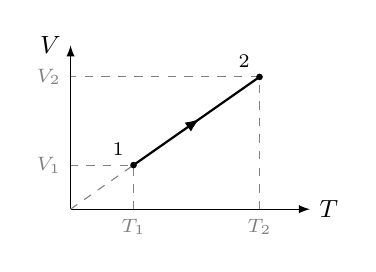
\begin{tikzpicture}[scale=0.8,>=latex]
  \draw[->] (0,0) -- (3.8,0) node[right] {\small $T$};
  \draw[->] (0,0) -- (0,2.6) node[left] {\small $V$};
  \draw[gray,dashed] (0,0) -- (1,0.7);
  \draw[gray,dashed] (1,0) node[below] {\scriptsize $T_1$} -- (1,0.7) -- (0,0.7) node[left] {\scriptsize $V_1$};
  \draw[gray,dashed] (3,0) node[below] {\scriptsize $T_2$} -- (3,2.1) -- (0,2.1) node[left] {\scriptsize $V_2$};
  \draw[thick,->] (1,0.7) -- (2.05,1.435);
  \draw[thick] (2,1.4) -- (3,2.1);
  \fill (1,0.7) circle (1.5pt) node[above left] {\scriptsize 1};
  \fill (3,2.1) circle (1.5pt) node[above left] {\scriptsize 2};
\end{tikzpicture}
\hspace{1.5cm}
\begin{tikzpicture}[scale=0.8,>=latex]
  \draw[->] (0,0) -- (3.8,0) node[right] {\small $T$};
  \draw[->] (0,0) -- (0,2.6) node[left] {\small $p$};
  \draw[gray,dashed] (0,1.5) node[left] {\scriptsize $p_0$} -- (1,1.5);
  \draw[gray,dashed] (1,0) node[below] {\scriptsize $T_1$} -- (1,1.5);
  \draw[gray,dashed] (3,0) node[below] {\scriptsize $T_2$} -- (3,1.5);
  \draw[thick,->] (1,1.5) -- (2.05,1.5);
  \draw[thick] (2,1.5) -- (3,1.5);
  \fill (1,1.5) circle (1.5pt) node[above] {\scriptsize 1};
  \fill (3,1.5) circle (1.5pt) node[above] {\scriptsize 2};
\end{tikzpicture}
\end{center}

\item
\begin{minipage}[t]{0.55\linewidth}
A grafikon $0\,^\circ$C-ról indul (a jég már olvadásponton van, nincs jégmelegedési
szakasz!). Először egy hosszú vízszintes szakasz következik (olvadás), majd egy ferdén
emelkedő egyenes szakasz $20\,^\circ$C-ig (a víz melegedése).

A vízszintes szakaszon a közölt hő a kristályrács felbontására, a molekulák közötti
kötések legyőzésére fordítódik: a belső energia nő, de a molekulák átlagos mozgási
energiája, így a hőmérséklet nem változik.

\emph{Arányok:} $L_\text{o}\approx 334~\text{kJ/kg}$, míg a víz melegítése
$20\,^\circ$C-ig $c\cdot 20\,^\circ\text{C} \approx 84~\text{kJ/kg}$, így a vízszintes
szakasz kb.\ négyszer olyan hosszú, mint az emelkedő.
\end{minipage}\hfill
\begin{minipage}[t]{0.40\linewidth}
\vspace{0pt}
\centering
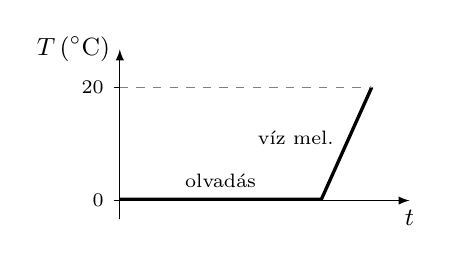
\begin{tikzpicture}[scale=0.8,>=latex]
  \draw[->] (0,0) -- (4.6,0) node[below] {\small $t$};
  \draw[->] (0,-0.3) -- (0,2.4) node[left] {\small $T$\,($^\circ$C)};
  \draw (0.1,0) -- (-0.1,0) node[left] {\scriptsize 0};
  \draw (0.1,1.8) -- (-0.1,1.8) node[left] {\scriptsize 20};
  \draw[very thick] (0,0.02) -- (3.2,0.02) -- (4.0,1.8);
  \draw[gray,dashed] (0,1.8) -- (4.0,1.8);
  \node[above] at (1.6,0.05) {\scriptsize olvadás};
  \node[left] at (3.55,1.0) {\scriptsize víz mel.};
\end{tikzpicture}
\end{minipage}

\end{enumerate}

\end{document}
